\documentclass{scrreprt}

\usepackage[utf8]{inputenc}
\usepackage{enumerate}
\usepackage[english]{babel} 
\usepackage{textcomp}

\usepackage{amsmath}
\usepackage{amsfonts}
\usepackage{amssymb}
\usepackage{amsthm}
\usepackage{mathtools}

\usepackage{graphicx}
\usepackage{wrapfig}
\usepackage{caption}

\usepackage[hidelinks]{hyperref}


\begin{document}

\title{Roux, an advanced approach to cubing}
\author{Dominic Zimmer}
\maketitle 

\tableofcontents
\chapter{Prologue}

\section{Abstract}
I'm going to introduce, explain and discuss a method to solve the Rubiks Cube called \emph{Roux}. I will assume the reader not to know how to solve the Rubiks Cube however the geometric understanding of the cube is required. Thus I will also mention some very basic information which might seem redundant to others.

\section{Perspectives}
Apart from Roux, there are plenty methods out there of which I will mention the most prevalent ones.

\begin{wrapfigure}{R}{0.4\textwidth}
\centering
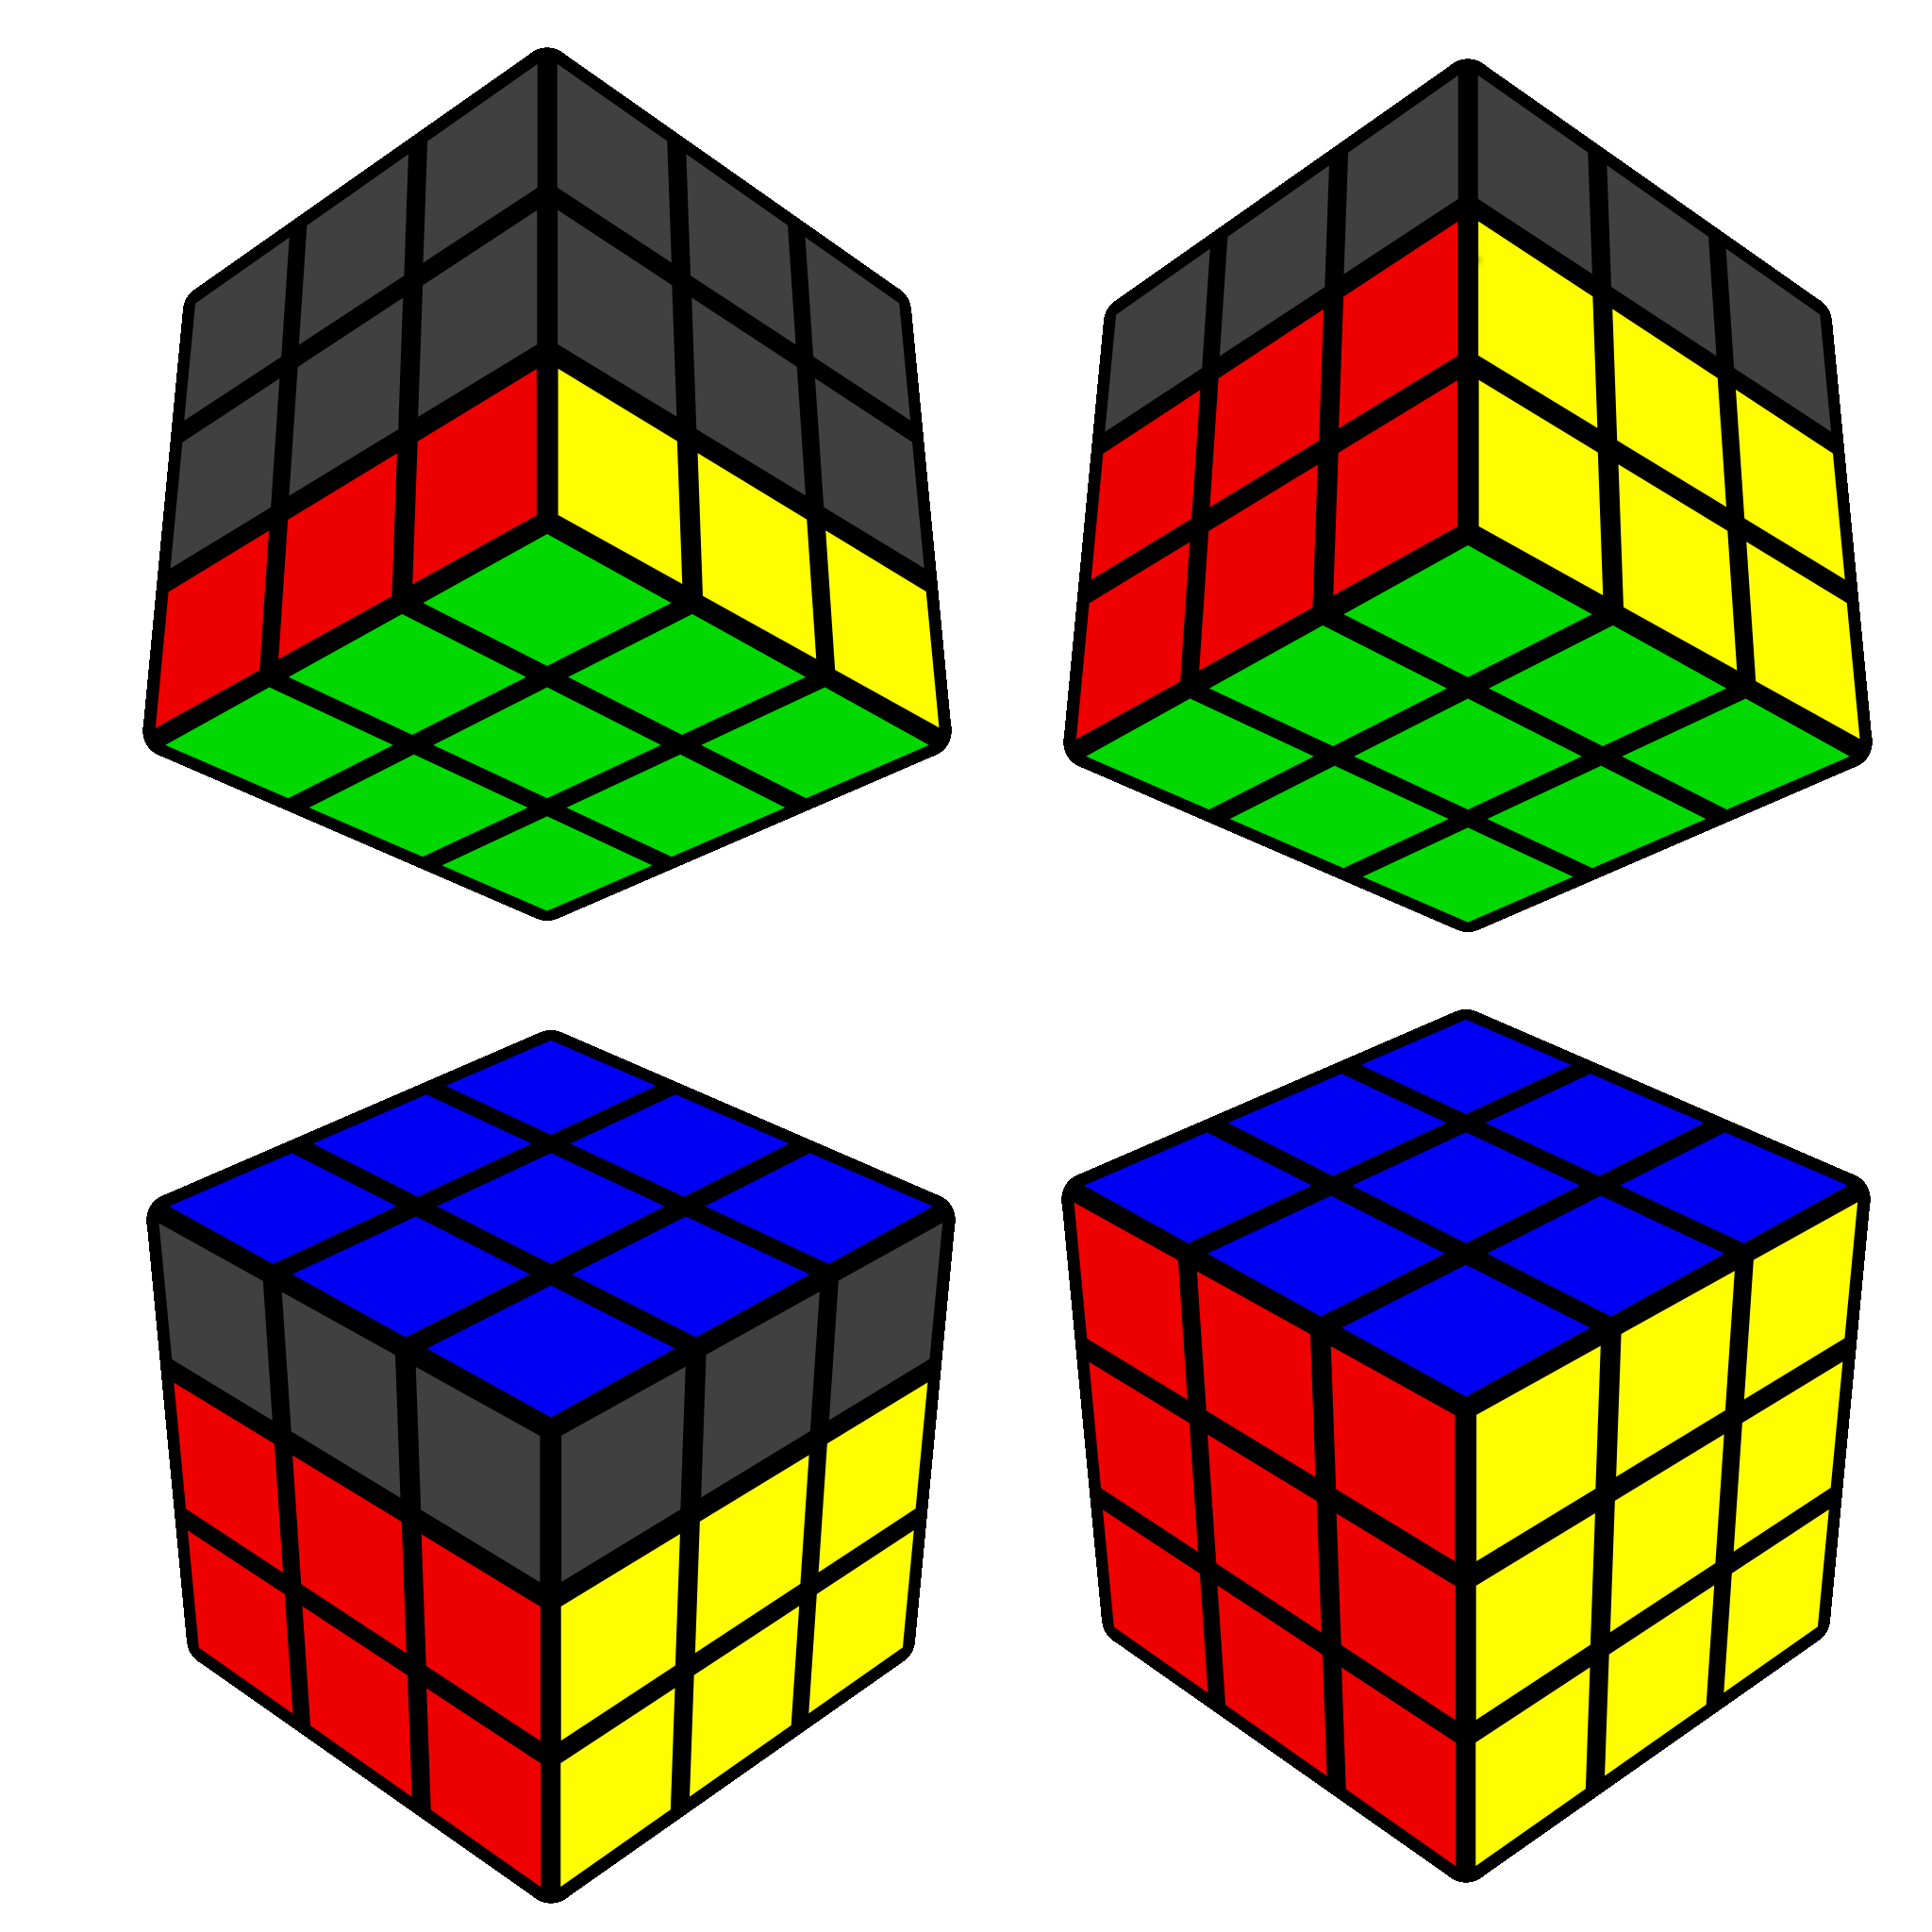
\includegraphics[width=0.3\textwidth]{union.png}
\caption*{The four steps of using the Beginners Method}
\end{wrapfigure}
First off, I am going to cover the \emph{Beginner's Method}, also known as \emph{Layer by Layer Method} which does what the name implies: it solves the cube layer by layer. This method seems pretty intuitive to most people as it starts off by solving one Face (which is easy to begin with). The most common method is closely related to the Beginner's Method: \emph{Fridrich's Method} or more commonly known as \emph{CFOP}. CFOP starts off by forming a \textbf{c}ross on one side, extending that cross to the \textbf{f}irst two layers, \textbf{o}rienting and \textbf{p}ermutating the last layer (leading to its unique name). You can see how closely related it is to the Beginner's Method: The key difference being that the Beginner's Method splits building the first two layers into two seperate steps whereas CFOP does this more efficiently. There are quite some more methods which deserve to be named here, for instance \emph{Petrus' Method}, but I'm going to leave it at that.


\section{Notation and terminology}
\subsection{Face turns}
To be able to communicate on this abstract level of thinking, we are going to use the standart notation and terminology which I will explain below.\par
In our notation we are not going to consider the colors of the individual facelets but rather keep the cube in one orientation. Thus we can easily refer to the six faces of the puzzle as \textbf{u}p, \textbf{f}ront, \textbf{r}ight, \textbf{l}eft, \textbf{b}ack and \textbf{d}own and abbreviate them each by their initial letter. Keeping that in mind, we intuitively define the moves \emph{U}, \emph{F}, \emph{R}, \emph{L}, \emph{B} and \emph{D} as clockwise 90\textdegree\ turns of their respective face.\par
To denote the counterclockwise turn of a side, we add an apostrophe to the respective turn. If we wanted to perform a 180\textdegree\ rotation of a face, we would simply append the number two to the move.


\subsection{Observations}
For clarification: we consider a the respective side of the cube to face us as we turn it: for instance \emph{U} and \emph{D} rotate opposite sides and turn in opposite directions. We certainly could also use \emph{U3} with the same logic as we defined \emph{U2} yet we would notice that \emph{U3} is the very same as \emph{U'}. We also see that \emph{R2} and \emph{R2'} result in the same turns, so would someoneone want to use \emph{R2'} at all? Yes - sometimes it can be useful to hint using two \emph{R'} moves over two \emph{R} moves for more comfortable turning. Note how we are using uppercase letters for the basic turns. Lowercase letters are reserved for an upcoming notation.

\begin{wrapfigure}{R}{0.3\textwidth}
\centering
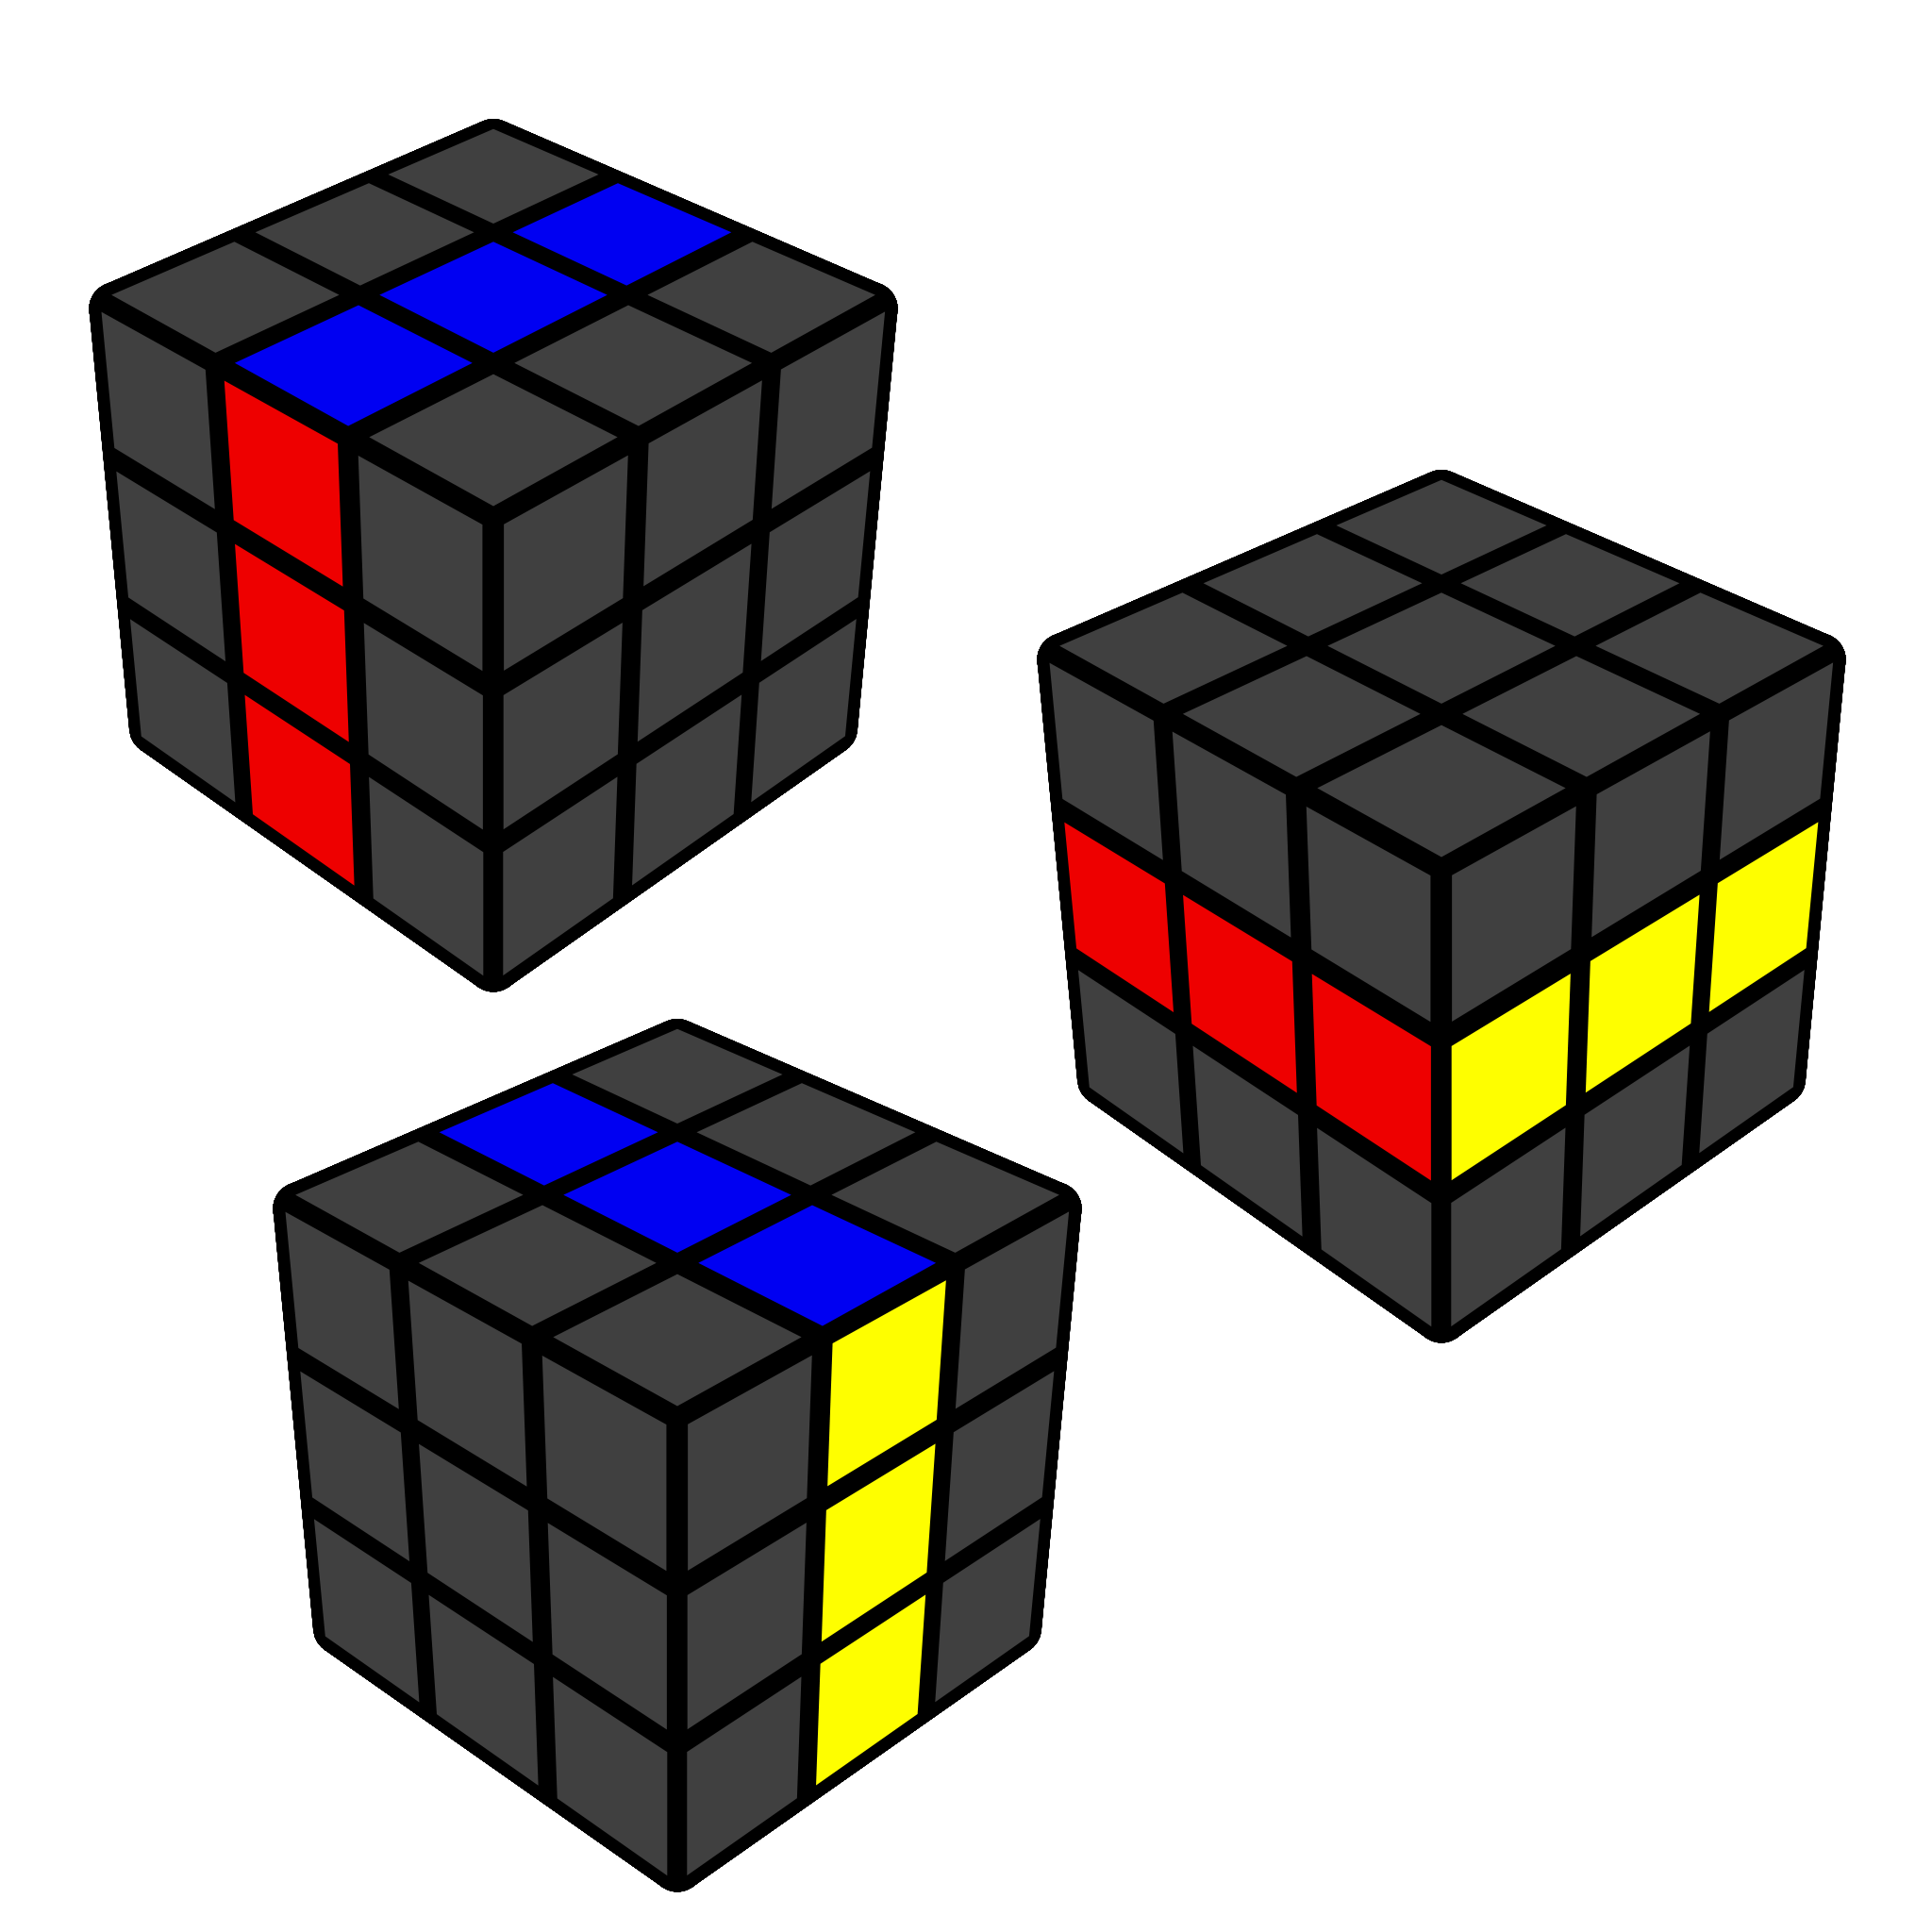
\includegraphics[width=0.25\textwidth]{slices.png}
\caption*{From top to bottom: the middle, equatorial and standing slice}
\end{wrapfigure}
\subsection{Slice turns, wide turns and cube rotations}
Sometimes the basic turns are inconvenient to use in a certain case, for instance if you wanted to turn the middle slice - the slice which is \emph{sandwiched} between the right and the left side. For that reason we define the \textbf{m}iddle slice turn, the \textbf{e}quatorial slice turn and the \textbf{s}tanding slice turn. We again abbreviate them respectively with their initials. However we need to declare that \emph{M} turns in the same direction as \emph{L}, \emph{E} turns in the same direction as \emph{D} and \emph{S} turns in the same direction as \emph{F}. Intuitively, we can append the earlier defined suffixes \emph{'} and \emph{2} with their corresponding interpretations.\par
For similar motivation as why we introduces the slice turns, we also define \emph{wide} moves. Wide moves are pretty self-explanatory: you grab two layers by expanding a face turn by the adjacent slice. We respectively add \emph{w} for \emph{wide} to our collection of suffixes. As we add more suffixes, we want to introduce an abbreviated form for wide moves: replacing the uppercase letter by a lowercase one.\par
The last notation we want to introduce are \emph{cube turns}. Cube turns require you to turn the entire cube inside your hands. We denote 	using the three axes \emph{X}, \emph{Y} and \emph{Z}.

\chapter{Roux}
Before we go into detail, I am going to give you a rough idea of how roux works.\par
\begin{wrapfigure}{R}{0.4\textwidth}
\centering
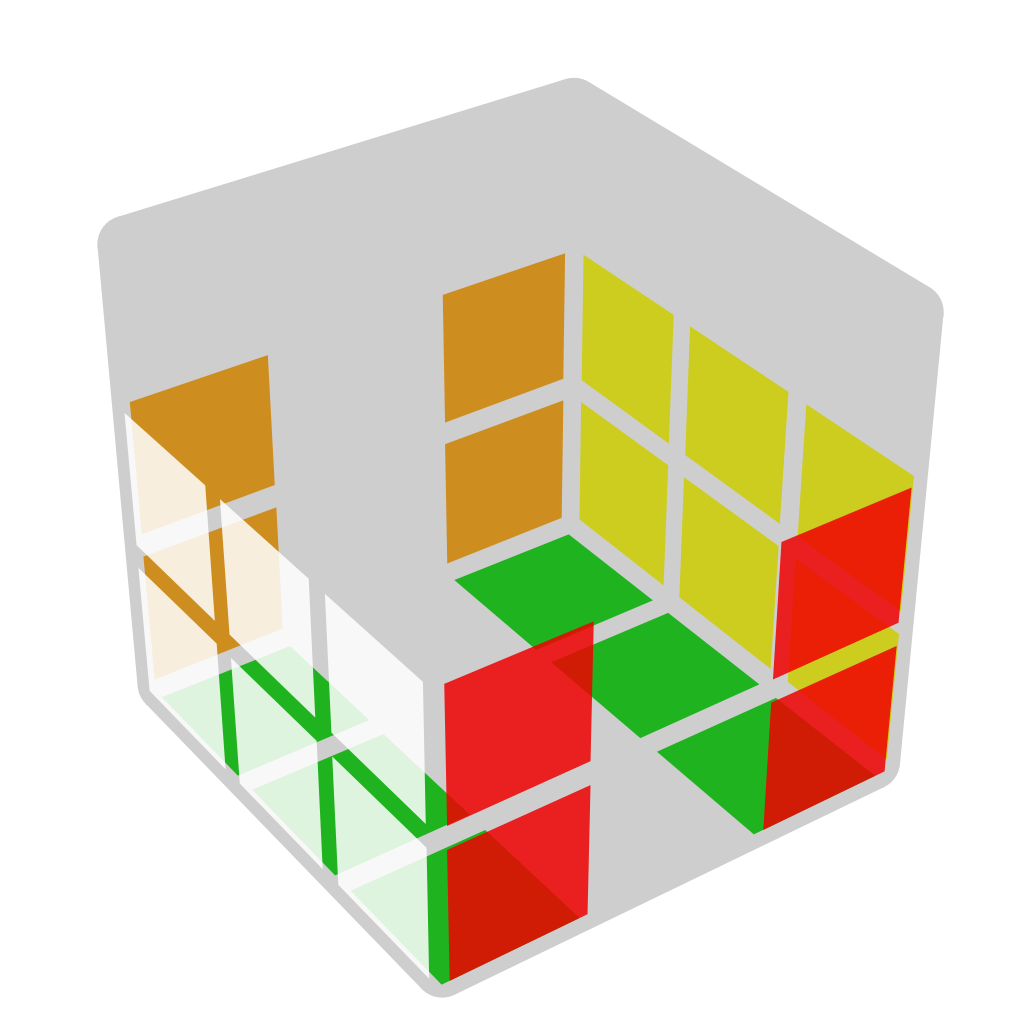
\includegraphics[width=0.4\textwidth]{f2b_transparent.png}
\caption*{The first Two Blocks }
\end{wrapfigure}
You start of by whats called the \emph{First Block}: you build a 1x2x3 block of one color around the matching center. Next up, we will mirror the first block onto the opposite side. This leaves us in the state of the \emph{First Two Blocks} already solved. We are left with "T"-shaped area which is yet to be solved. Notice how every piece that is yet to be solved is on either the middle slice or the upper layer. Mathematicians like to call this area the \emph{span}, denoted as $\langle M, U \rangle$, of \texttt{U} and \texttt{M}.\par
\begin{wrapfigure}{L}{0.4\textwidth}
\centering
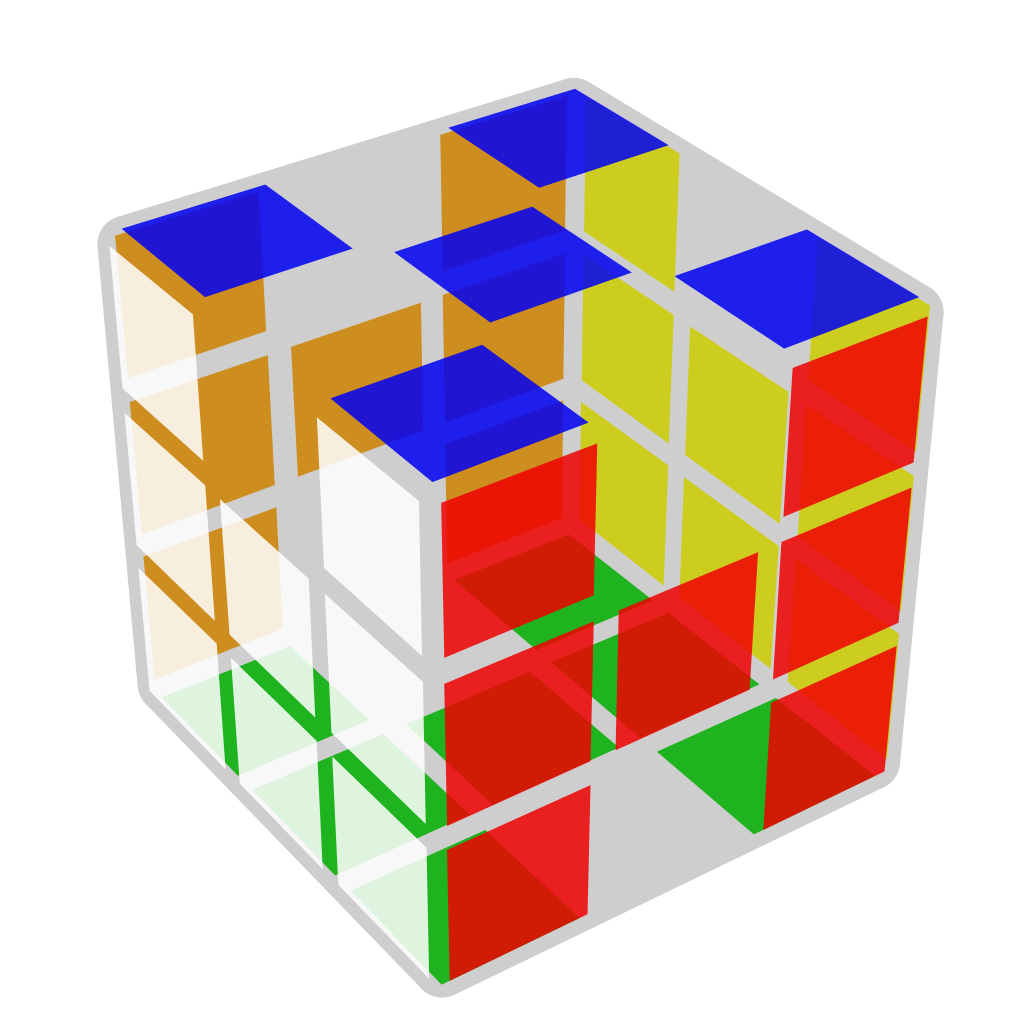
\includegraphics[width=0.4\textwidth]{lse.png}
\caption*{Before the Last Six Edges}
\end{wrapfigure}
We now want to solve the corners of the upper layer to be left with six unsolved edges and four unsolved centers. Solving the corners of the upper layer will be split into two seperate steps: first we orient the corners to have their common color face up, then we permute them to the places where they belong. Both of these steps are not very trivial and thus will require some algorithms.\par
As mentioned previously, we are now left with six edges and four centers unsolved. As you realize quickly, the centers are at most two \texttt{M}-slice moves from being solved, leaving us with the \emph{Last Six Edges}. As you can see in the figure beside



\section{First block}

\section{Second block}

\section{Corners Last Layer}

\section{Last six edges}

\chapter{Appendix: Algorithms}

\section{2 Look CLL}

\section{CMLL}

\section{LSE}


\end{document}